\documentclass[a4paper,10pt]{book}

\usepackage[utf8]{inputenc}
\usepackage[english]{babel}
\usepackage{graphicx}
\usepackage{float}
\usepackage{geometry}
\geometry{margin=3cm}

\newcommand{\quotes}[1]{``#1''}
\newcommand\tab[1][1cm]{\hspace*{#1}}

%opening
\title{\textbf{TX52 - scientific project report }\\
  Create a Real-Time Strategy Game Engine with SARL, an agent oriented language}
\author{~\\
  \textbf{Olivier Villequey, Romain Dulieu} }

\begin{document}

\maketitle

\tableofcontents

\chapter{Project Definition}

\section {Introduction}

~

The goal of this project is to create a Real-Time Strategy (RTS) game engine.

Firstly, we have to define what is a RTS game and what are the important specificities or components of this kind of games :
\begin{itemize}
 \item Real-time strategy : include an enormous number of possible game actions that can be executed at any given time. The result or effect of any action is unknown
  and changes as the time goes by. Furthermore, RTS games usually manipulate a large number of units, controlled by an AI, which is an important aspect of our project. 
 \item We consider that RTS games include only partially observable environments. It means that one aspect of the strategy is to collect informations by exploring the environment.
 \item A map : an environment composed of different objects static (walls, trees, cliffs, etc.) or dynamic (units) with specific 2D/3D environment features such as the topography etc.
 \item Different types of AIs : strategic level or global AI that takes abstract decision making to achieve the main goal : deciding the size of the force necessary to move/attack a position, the kind of forces needed ... 
  On the other hand, the tactical level or local AI concerns more concrete decisions (handle the actions : moving,attacking,producing ...) and is responsible for achieving the objectives defined at the strategic level.
\end{itemize}

With all these informations in mind we have to determine which technology we will use to  implement the game engine. We choose the SARL language, an agent oriented language based on Java. We think that the agent-oriented approach seems the one that permit to answer to a lot of constraint easily.

In this report we will firstly make a summary of what others people may have done in this field of research through a State of the art. Secondly, We will explain how our engine work with a complete description of the architecture we designed. Then we will show you a small example of what it's possible to create with this engine. Lastly, we will develop the performance aspect of the engine with benchmarks.



\newpage

\section {State of the art}

~

First of all, as the gaming tools and games are developed in private companies it is difficult to get recent public papers about the actual technologies used in RTS games. 
That's why our sources may be a little bit old but it is easier to find public sources from a couple of years ago.

~

\subsection{RTS history}

~

Real-time strategy (RTS) games are known to be one of the
most  complex  game  genres  for  humans  to  play,  as  well  as
one  of  the  most  difficult  games  for  computer  AI  agents  to
play well.  To tackle the task of applying AI to RTS games,
recent techniques have focused on a divide-and-conquer approach, 
splitting the game into strategic components, and developing 
separate systems to solve each. This trend gives rise
to  a  new  problem:   how  to  tie  these  systems  together  into
a functional real-time strategy game playing agent.

~

Traditional games such as Chess and Go have for centuries
been  regarded  as  the  most  strategically  difficult  games  to
play at a top level. High-level play involves complex strategic
decisions  based  on  knowledge  obtained  through  study
and  training,  combined  with  online  analysis  of  the  pieces
on the current board.  Top players are able to “look ahead”
a dozen or more moves into the future to decide on an
action, often under strict time constraints, with clocks for each
player ticking away as they think make their decision.  Let
us now imagine a genre of game in which the playing field
is 256 times as large, contains up to several hundred pieces
per player, with pieces able to be created or destroyed at any
moment.  On top of this, players may move any number of
pieces simultaneously in real-time, with the only limit being
their own dexterity.   What we have just described is a
real-time strategy (RTS) game, which combines the complex
strategic elements of traditional games with the real-time 
actions of a modern video game.

~

A relatively new genre, the first RTS games started to appear
in  the  early  1990s  with  titles  such  as  Dune  II,  
WarCraft,  and Command and Conquer.   Originally introduced
as a single-player war simulation, their popularity exploded
as the internet allowed for players to compete against each
other in multiplayer scenarios. With the creation of StarCraft
in 1998, RTS games had reached a level of strategy unseen
in other video game genres.

~

\subsection{Environment}

~

RTS games take place on a map, composed of a finite or infinite number of cells with a position organized in a grid. On this basis,
you can choose to create a continue or discontinue environment space. Most of the RTS are still based on a two-dimensional map even 
in 3D engines. In fact, newer games didn't innovate much on the initial concept but tend to emphasize more on the basic RTS elements
such as higher unit cap, more unit types, larger maps, etc.
Environments can implement climate changes, different types of terrain that impact certain types of movement etc.

~


\subsection{Path Finding}

~

Path finding is the ability for the agent to find his way from his position to a destination by taking the shortest path and of course avoiding the obstacles between him and the destination position.
In most commercial RTSs, the solution for the path finding is using A* over a navigation mesh (commonly referred to as a \quotes{navmesh}). Navmesh is used to create the nodes of our graph by creating polygons	on the surface area where the agents can move. This can be hard coded and so labour intensive or it is possible to create an algorithm that generate the navmesh from a given map.
When the navmesh is created, you can apply A* algorithm on the graph to determine the shortest path.
To do so, here is a short explanation of how A* algorithm works:
\begin{itemize}
 \item Create two lists : CLOSED for the nodes already evaluated and OPEN for the ones to be evaluated. Add the starting node to the OPEN list.
 \item A loop : select the lowest cost node in open and move it to the CLOSED list
 \item \tab if the node is the target then it's over
 \item \tab for each neighbour of the selected node, if it is in CLOSED skip to the next neighbour
 \item \tab \tab if the new path to neighbour is shorter or neighbour is not in OPEN then set his new path cost and set the current node as its parent
 \item \tab \tab if neighbour is not in OPEN add neighbour to OPEN.
 \item	\tab end of for
 \item end of loop
\end{itemize}
             
~

\subsection{AIs in RTS}

~

Inspired by  military command structures,  tasks are partitioned among modules
by their intuitive strategic meaning (combat, economy, ...),
with vertical communication being performed on a “need to
know” basis.  High level strategy decisions are made by the
global AI by compiling all known information about
the current game state.  Commands are then given to local AI
which are directly in charge of completing the low-level task.

~

\textbf{References} 
\textit{\\Incorporating Search Algorithms into RTS Game Agents},
David Churchill and Michael Buro

\subsection{Analysis}

~

After doing these research on the RTS games in computer science we are able to see what are main issues that we find in existing solutions to our problem.

First of all, the difficulty to find sources of modern engine is obviously a main issue but this problem can be solve easily for our project.

Secondly, the number of units actives at the same time is an obstacle that our engine must overcome. We will have to implement an environment as efficient as possible.

Thirdly, with an agent-oriented solution we will be able to simulate a powerful general without making it omniscient. That's why we decided that all units will be an agent and they will follow order and communicate with other.

To conclude, because of the oriented agent design that we choose our solution is different from what we find in other research works. This is the opportunity to build a solution that can answer the problem in a more modern way.

~

\newpage
\chapter {Models}

~

\section {Architecture}

~

Our program is divided in three major parts :
\begin{itemize}
 \item The environment, written in Java, that contains the world we created as well as the Jbox2D world that solve the physics
 problems. Both worlds will coexist in the main class Environment.
 \item The agent part, written in SARL, with all agents : the Environment Agent, the main controller of the game engine. It
 communicates with the Environment, all the units and the GUI. It coordinates their actions and leads the main cycle of the game.
 Then, there are the Units Agents with their bodies in the environment and the possibility to act with some behaviours corresponding to
 their perceptions.
 \item The Graphical User Interface, written in Java using Swing libraries. We didn't choose the best solution to do the GUI as
 we don't have much experience with JavaFX and so we chose to use Swing because it was easier for us and finally the GUI wasn't the most
 important objective of our project.
\end{itemize}

~
\newpage
\section {UML}
\subsection{Environment class diagram}
~

Firstly, the diagram below shows the class diagram of the environment :

~

\begin{figure}[!ht]
 \parshape1 -2.5cm 21cm
 \centering
 \includegraphics[scale=0.5]{TX52UML}
 \caption{Environment Class Diagram}
\end{figure}
\parshape0

~

The center class is of course Environment with both Jbox2D world and the world we created. it also contain the list of events from the listeners of the environment, more precisely the GUI in our project.

Jbox2D contains the objects and is used to handle the physics whereas EnvMap is the world we made with a QuadTree algorithm that contains all the objects, methods to add or remove objects and the list of bodies of all the units. This tree is dynamic and his update is managed by an iterator optimized for this kind of structure in the function "updateTree".

~

All the objects are Environment Objects, they can be Static (walls, obstacles etc) or Dynamic (units). AgentBody is an example of a unit that we added with a specific perceptionDistance, attack speed, life and also its team. The "box" of each object is a MinimumBoundingRectangle containing the body of the agent that is calculated dynamically when we need it.
In addition, each Environment Object is characterized by a semantic enumeration that represent the exact type of object. With this system you don't need to extend the static or dynamic object class to create new types in the world.

~

Lastly, within their perception range, agents have a list of Perceivable which contains the ID of the object and several information that will be used to decide its following influence. Also, EnvironmentChangeQuery is used to communicate with the environment agent and transmit the next influence.

~

\newpage
\subsection{Agents class diagram}

The following UML shows the agent part mostly written in SARL :

~

\begin{figure}[!ht]
 \parshape1 -2.5cm 21cm
 \centering
 \includegraphics[scale=0.6]{TX52AgentUML}
 \caption{Agent Class Diagram}
\end{figure}
\parshape0

The agent part wasn't the main part of the project so we implemented only the essential classes.

The EnvironmentAgent is here to coordinate all others agent and guarantee that the simulator run smoothly. It communicates with the others agent through the EventBlock.
All important function are implemented under the form of skills following the SARL mentality. 

In order to implement agents you need to extends the Agent class. You can create behaviours in order to personalize the comportments of your agents. Agents can send two kinds of influences, Motion or Shoot in function of the desired action.

This sequence diagram explains how cycles are executed and shows interactions between agents.

\begin{figure}[!ht]
 \parshape1 -2.5cm 21cm
 \centering
 \includegraphics[scale=0.6]{TX52SeqDiag}
 \caption{Sequence Diagram}
\end{figure}
\parshape0

\newpage
\section {Installation and Warnings}

~

In order to use this engine you have to download the sources files. You can find them on the gitHub of the project : https://github.com/OlivierVillequey/TX52-StrategyGameEngine

Use SARL eclipse IDE and add to build path the .jar of Jbox2D-library and AFC-math package.

If you decide to program yourself new agents there are some rules to follow : 
\begin{itemize}
\item all your agents must send one and only one influence when their receive a Perception.
\item all your agents must receive one and only one perception at each step of simulation.
\item if you want your agent to doesn't move or act during a step use the "doNothing" function
\item at the end of the initialisation of your agent don't forget to send an event "AgentReady" to the environment.
\end{itemize}

~
\newpage
\chapter {Application}

~

In this section, we will show the window of our application. Firstly the map :

~

\begin{figure}[h]
 \centering
 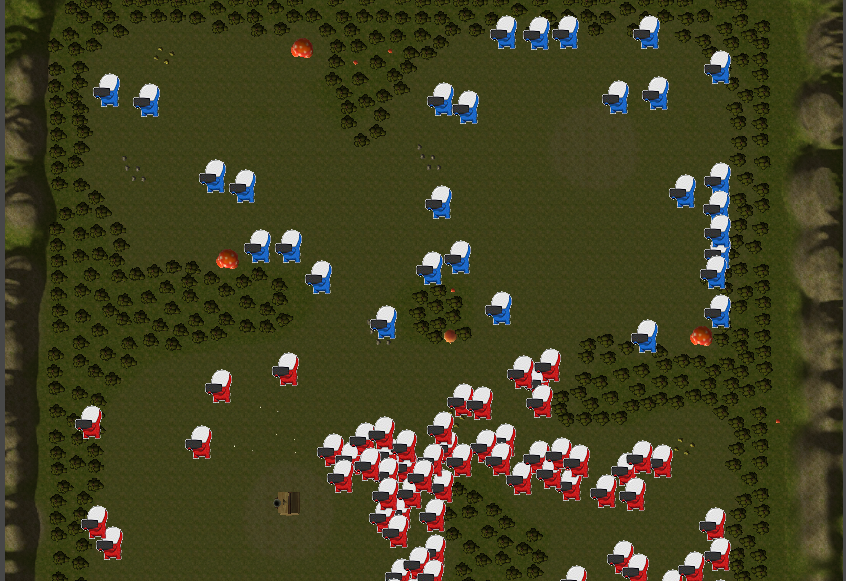
\includegraphics[scale=0.5]{GUI2}
 \caption{map}
\end{figure}

~

Like you can see the color of the unit shows the team and our units randomly walk around the map until they are in range of an enemy unit and stops to start shooting. Units are spawn at a constant rate in one corner of the map.

~

We added the possibility to spawn new units for each team on the right side with a spawn button :

~

\begin{figure}[h]
 \centering
 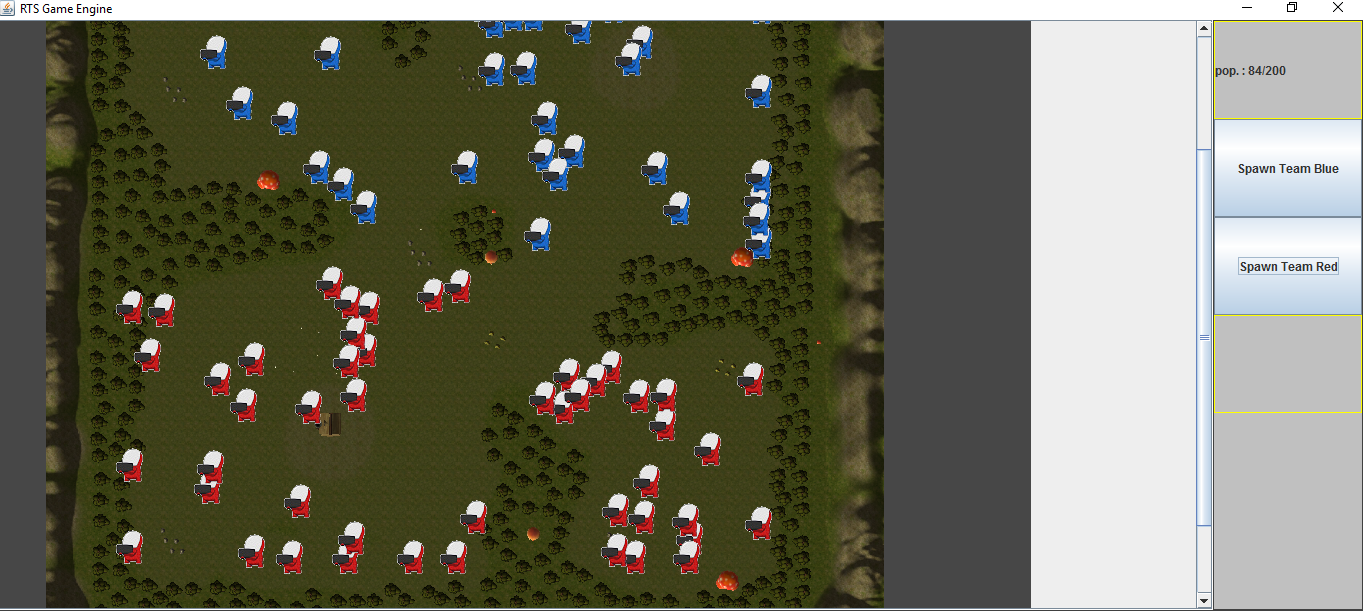
\includegraphics[scale=0.5]{GUI3}
 \caption{Screenshot of the application window}
\end{figure}

For this example we created a class AbstractAnimat that contains all requirements to communicate with the world. All units are an instance of the agent "AgentTest" that extends this class. A lot of used function are skills and can be found in the file "skill.sarl".

\newpage

\chapter {Performance}

~

In this section, to test the performance of our program we tried to see the evolution of the elapsed time of some key functions. The conditions will always be the same : we spawn 1 agent at every step and we look at the 500 first steps of the execution.

~

The first one is the function that resolves influences :

\begin{figure}[h]
 \centering
 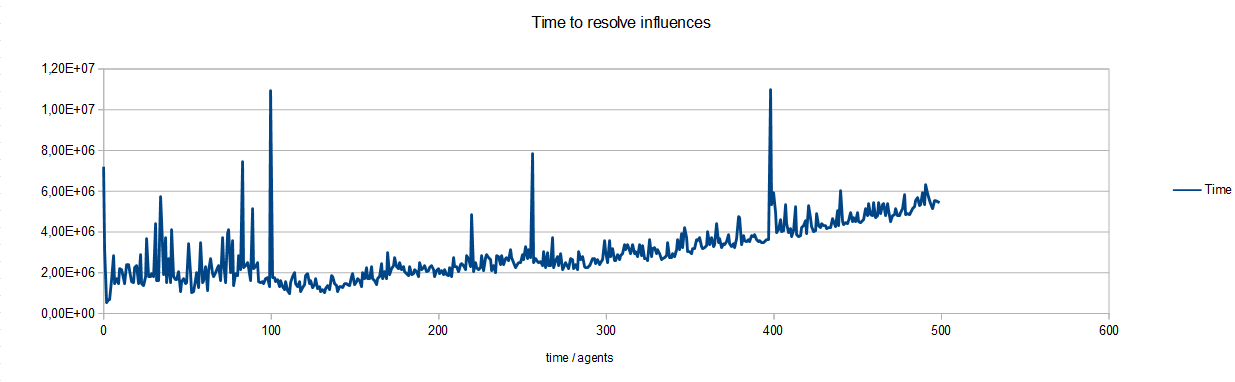
\includegraphics[scale=0.5]{resolveInfluence}
 \caption{Elapsed time of resolveInfluence()}
\end{figure}

We can see that the results are satisfying with an average time around $2.5\times10^{-6}$ s.

~

The next one is about the updateTree() function :

\begin{figure}[h]
 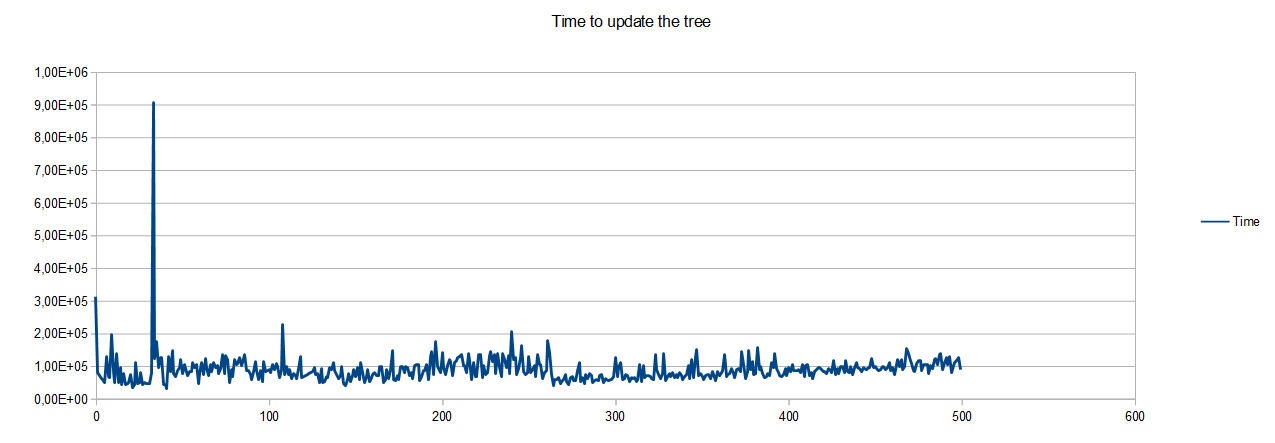
\includegraphics[scale=0.5]{updateTree}
 \caption{Elapsed time of updateTree()}
\end{figure}
Here, the elapsed time is more stable overall but we can notice big spikes occasionally that are 9 times longer than the average value of $1.0\times10^{-5}$ s. We didn't find any explanation on the reason why it happens.

\newpage

For the third test, we are looking at updateWindow(), it is the most time consumming function and we faced some difficulties to improve the performance and manage to display a large number of units without any spikes. At this point, the window can display until 300 units before slowing down the framerate.

~

\begin{figure}[h]
 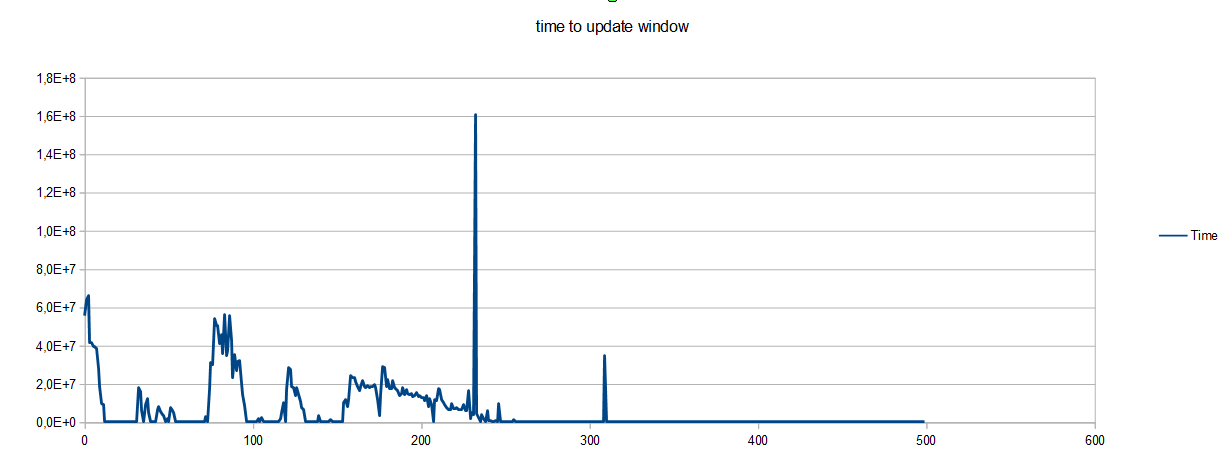
\includegraphics[scale=0.5]{updateWindow}
 \caption{Elapsed time of updateWindow()}
\end{figure}

~

Problem: the results are unexpected because as much as time goes by and the number of units increase the time computed is shorter, the explanation we assumed is that the window has a separate thread from the main cycle and so the execution doesn't wait that the window has refreshed before continuing the cycle.

\chapter {Conclusion}

In this research project we made an application almost from scratch. It was an intense and interesting experience for both of us. We had to document ourselves of the state of the research in this, design an engine and implemented it. Thanks of the previous works and the help of Stephane Galland our tutor this project was easier to accomplish. 

We are pretty happy of the performance that engine provide but if we had more time we would improve some points. For example, there is no path finding yet in the engine. It's some work that the user must do himself for now. Even if the engine is efficient for now we think that there are still some little things that could be improved.


\end{document}
